\section{Мета практикуму}

Практично ознайомитися із принципами баєсівського підходу в криптоаналізі,та безпосерденьо побудувати детерміністичну та стохастичну матриці для заданих розподілів. 


\subsection{Постановка задачі та варіант}
\begin{tabularx}{\textwidth}{X|X}
	\textbf{Треба виконати} & \textbf{Зроблено} \\
	Описати побудову алгоритму & \checkmark \\
	Порахувати таблицю ймовірностей $P(\textit{M}|\textit{C})$ & \checkmark \\
	Показати детермінитичну та стохастичну функції & \checkmark \\
	Порахувати середні витрати для вирішуючих функцій & \checkmark \\
\end{tabularx}



\section{Хід роботи/Опис труднощів}
    Для виконанння лабораторної роботи була обрана мова програмування Python та бібліотека для роботи з таблицями Pandas, написані функції для отримання розподілу шифротекстів та сумісного розподілу відкритих текстів та шифротекстів. 
    
    З цього було отримано відповідні таблиці ймовірностей, яких вже були побудовані детерміністичну та стохастичні функції, а також обраховані середні втрати. 
    
    Під час виконання роботи виникли труднощі з певною невідповідністю формату даних при їх завантаженні у код, тому на початку було застосовано деякий препроцесінг з вхідними даними та отримано зручні для роботи таблиці.


\section{Результати дослідження}
У ході роботи було визначили, що детерміністична та стохастична вийшли не однаковими, але обоє значень серденьої похибки у обох функцій вийшли однаковими. У результаті отримали, що ніякій із функцій надати перевагу не можемо, вони обоє добре підходять для нашого розподілу.

\subsection{Опис алгоритму}
Для побудови детерміністичної функції та стохастичних функцій наведемо наступний алгоритм.

\begin{remark}
	Одразу зазначимо, що алгоритми подібні та відрізняються лише у останньому кроці. Для послідовності опису наведемо повні кроки. 
\end{remark}

\begin{algorithm}
    \begin{enumerate}
    	\item Алгоритм із побудови детерміністичної вирішуючої функції.
    		\begin{itemize}
       		 \item Обчислюємо $P(C)$ за формулою: $\forall C: P(C) = \sum_{(M, k): E_k(M) = C} P(M, k)$.
        		\item Обчислюємо $P(M,C)$ за формулою: $\forall (M, C): P(M, C) = \sum_{k: E_k(M) = C} P(M, k)$. 
        		\item Обчислюємо $P(M|C)$ за формулою $\dfrac{P(M,C)}{P(C)}$.
        		\item Із обчислених значень умовних ймовірностей вибираємо максимальні значення. Та присвоюємо $1$ до тих комірок у матриці де зустріли його.
    		\end{itemize}

    	\item Алгоритм із побудови стохастичної вирішуючої функції.
    		\begin{itemize}
       		 \item Обчислюємо $P(C)$ за формулою: $\forall C: P(C) = \sum_{(M, k): E_k(M) = C} P(M, k)$.
        		\item Обчислюємо $P(M,C)$ за формулою: $\forall (M, C): P(M, C) = \sum_{k: E_k(M) = C} P(M, k)$. 
        		\item Обчислюємо $P(M|C)$ за формулою $\dfrac{P(M,C)}{P(C)}$.
        		\item Із обчислених значень умовних ймовірностей вибираємо макимальні значення. Та у тих рядках, де максимальне значення повторюється $s$ разів присвоюємо коміркам значення $\dfrac{1}{s}$. 
    		\end{itemize}
	\end{enumerate}
\end{algorithm}


\subsection{Таблиця ймовірностей}
Таблиця ймовірностей набула наступної форми.

\begin{figure}[h]
    \centering
    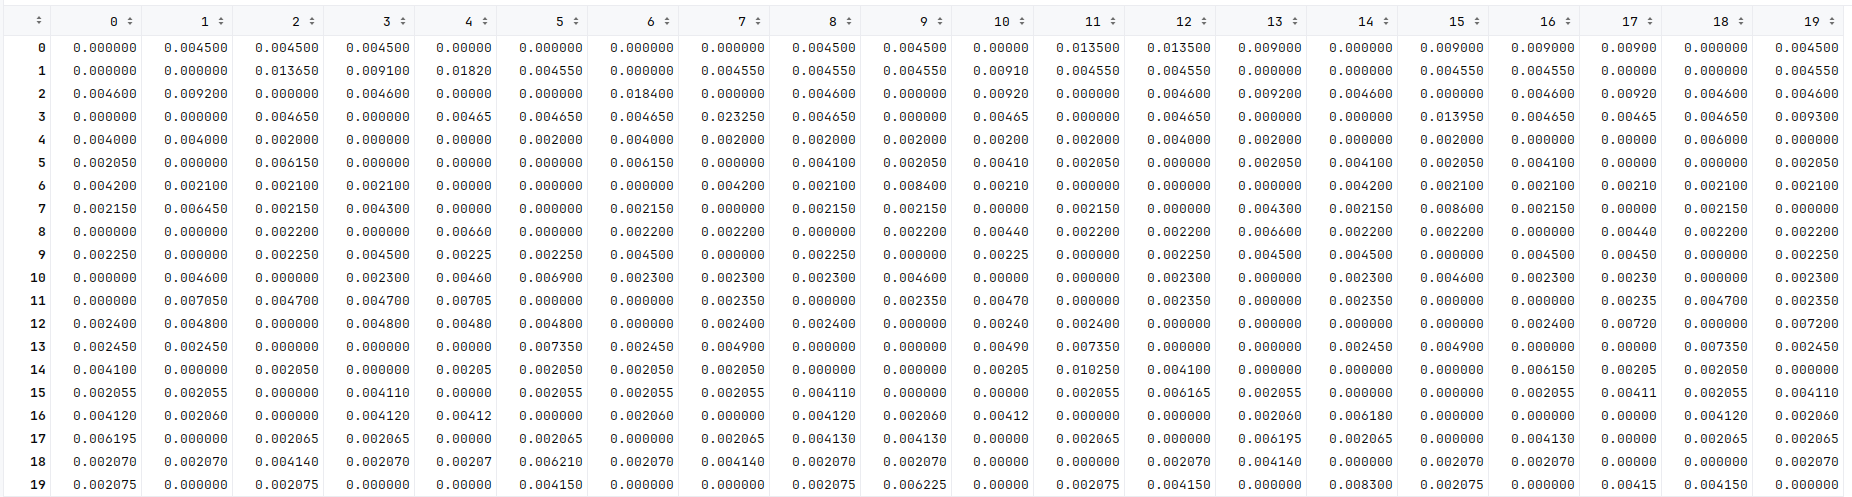
\includegraphics[scale = 0.25]{Images/conditional_prob}
    \caption{Таблиця умовних ймовірностей для обчислення вирішуючих функцій.}
    \label{fig:twisted_edward}
\end{figure}


\subsection{Детерміністична та стохастична матриці}
У ході обчислень було отримано наступні функції.

\begin{figure}[h]
    \centering
    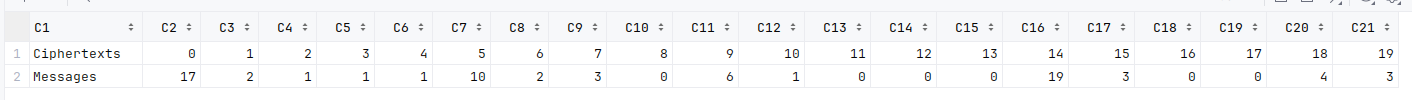
\includegraphics[scale = 0.34]{Images/deterministic}
    \caption{Детерміністична вирішуюча функція зображена у формі відображень. (ШТ $\shortrightarrow$ ВТ) }
    \label{fig:twisted_edward}
\end{figure}

\begin{figure}[h]
    \centering
    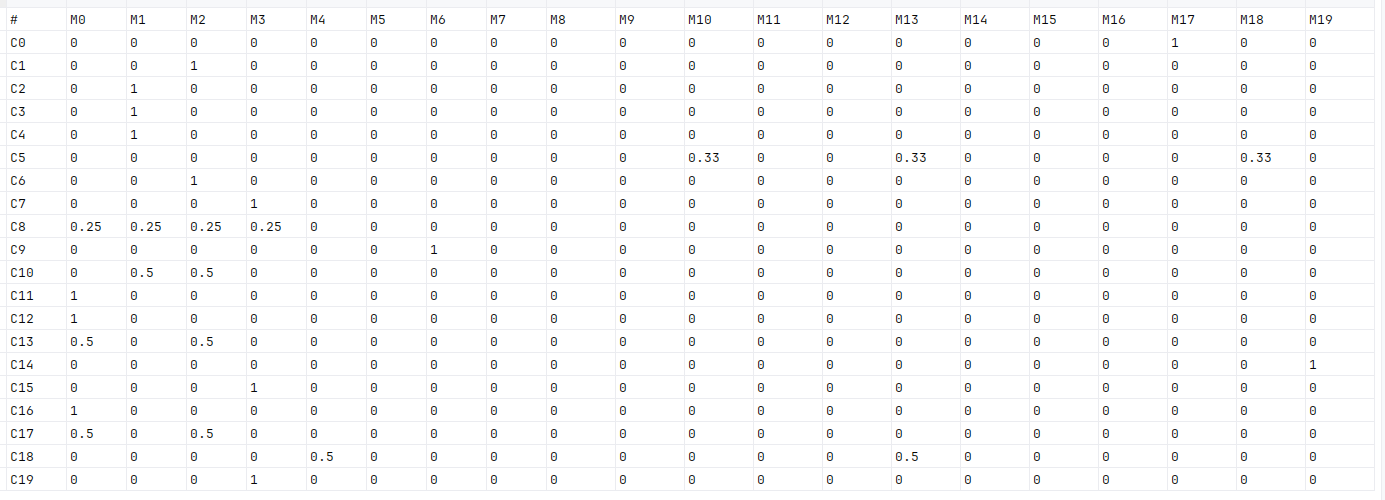
\includegraphics[scale = 0.3]{Images/stochastic}
    \caption{Стохастична вирішуюча функція.}
    \label{fig:twisted_edward}
\end{figure}

Також серденє значення втрат вийшло таким:
\begin{itemize}
	\item Для детерміністичної вирішуючої функції значення втрат становить: $0.786$.
	\item Для стохастичної вирішуючої функції значення втрат становить: $0.78599$.
\end{itemize}

\newpage

\section{Висновки}
За допомогою реалізації практикуму ''Баєсiвський пiдхiд в криптоаналiзi: побудова i дослiдження детермiнiстичної та стохастичної вирiшуючих функцiй'' дізналися на практиці як повинен відбуватися баєсівський підхід у криптоаналізі. Також були долучені до створення такого собі <<маленького>> прикладу із побудови вирішуючих функцій для заданого розподілу повідомлень.
